\chapter[The 22$^{\text{nd}}$ of March 2024 - 2D and Orthogonality discussion]{2D and Orthogonality discussion}
\label{Chap_22_03_24}
\begin{chapabstract}
    This week the 2D has drastically moved forward and some investigations on the orthogonality were made. 
\end{chapabstract}

\minitoc

\section{2D}

The mixed formulation with T3 elements works. Quadratic elements are on the way

\section{Orthogonality}
\label{sec:orthogonality}
 In order for the loss implementation not to somehow bring back the curse of dimensionality it is important to rely on the tensor decomposition and not compute the full order tensors. However, it does not seem easy to remove the full tensors field evaluation to compute the integral due to the square of the gradient 
 \begin{equation}
     \left( \frac{\partial u}{\partial x} \right)^2 = \left( \sum\limits_{i=1}^m \textcolor{BleuLMS!70}{\frac{\mathrm{d}\overline{\vect{u}}_i(\vect{x}) }{\mathrm{d}x}} ~\textcolor{LGreenLMS}{\prod_{j=1}^{\beta}\lambda_i^j(\mu^j)} \right)^2.
 \end{equation}
 To do so an idea could be to try to rely on  the orthogonality of the space modes.
 
\subsection{Post processing Gram-Schmidt}
So as not to modify the interpolation given by the NN, it appears less intrusive to solely modify the post-processing of the interpolated field before computing the loss.

\subsubsection{One extra parameter}
An orthogonalisation step can be carried out in the case of a single extra-coordinate. This step allows the previously computed modes to form a basis without losing the newly computed information. Moreover, projecting a new mode onto the basis provides additional insights: the extent to which it adds new information. For instance, if its projection is zero, it indicates that the previous modes already represent this mode, rendering it irrelevant. In practical terms, for each pair of modes $\left(\overline{\vect{u}}_{m+1},\lambda_{m+1}\right)$, we ``eliminate" from $\overline{\vect{u}}_{m+1}$ the projection of the new mode onto the preceding modes, yielding $\mathring{\overline{\vect{u}}}_{m+1}$. Consequently, we adjust the $\lambda_{i}$ values accordingly to avoid information loss, resulting in $\mathring{\lambda}_i$. Subsequently, we normalise this new mode $\mathring{\overline{\vect{u}}}_{m+1}$ using equations (\ref{ortho}), (\ref{normaliz1}), (\ref{normaliz2}), and (\ref{normaliz3}).
	
	\begin{equation}\label{ortho}
		\vect{u}_{m+1} = \sum_{i=1}^{m} \underbrace{(\lambda_i + \lambda_{m+1} ~ \overline{\vect{u}}_i^T  \overline{\vect{u}})}_{\mathring{\lambda}_i} \overline{\vect{u}}_i + \lambda_{m+1} \underbrace{\left(\overline{\vect{u}}_{m+1} - \sum_{i=1}^{m} ( \overline{\vect{u}}_i^T  \overline{\vect{u}}) \overline{\vect{u}}_i\right)}_{\mathring{\overline{\vect{u}}}_{m+1}}
	\end{equation}
	
	\begin{equation}\label{normaliz1}
		\overline{\vect{u}}_{m+1} \longleftarrow \frac{\mathring{\overline{\vect{u}}}_{m+1}}{\Vert\mathring{\overline{\vect{u}}}_{m+1} \Vert_{\ftensor{K}}}
	\end{equation}
	
	\begin{equation}\label{normaliz2}
		\lambda_{m+1} \longleftarrow \lambda_{m+1} \Vert\mathring{\overline{\vect{u}}}_{m+1} \Vert_{\ftensor{K}}
\end{equation}
\begin{equation}\label{normaliz3}
	\{\lambda_i\}_{i\in\llbracket1,m\rrbracket} \gets \{\mathring{\lambda}_i\}_{i\in\llbracket1,m\rrbracket}
\end{equation}
\Rq{Alternatively, time vectors can also be compressed as proposed in \parencite{giacoma_toward_2015}, converging towards the SVD decomposition of the displacement field, thus avoiding redundancy in temporal vectors.}


\subsubsection{Multiple extra parameters}

The modified Gram-Schmidt algorithm that allows keeping the same solution field after and before the orthonormalisation process is not applicable in case of more than 1 extra parameter. Indeed, orthogonalising the mode $m+1$ with the previous basis without loosing information amounts to writing 
	\begin{equation}\label{ortho}
		\vect{u}_{m+1} = \sum_{i=1}^{m} \underbrace{(\lambda_i^{(1)}\lambda_i^{(2)} + \lambda_{m+1}^{(1)}\lambda_{m+1}^{(2)} ~ \overline{\vect{u}}_i^T  \overline{\vect{u}})}_{\neq \mathring{\lambda}_i^{(1)}\mathring{\lambda}_i^{(2)}} \overline{\vect{u}}_i + \lambda_{m+1}^{(1)}\lambda_{m+1}^{(2)} \underbrace{\left(\overline{\vect{u}}_{m+1} - \sum_{i=1}^{m} ( \overline{\vect{u}}_i^T  \overline{\vect{u}}) \overline{\vect{u}}_i\right)}_{\mathring{\overline{\vect{u}}}_{m+1}}.
	\end{equation}
In the general case, 
\begin{equation}
    (\lambda_i^{(1)}\lambda_i^{(2)} + \lambda_{m+1}^{(1)}\lambda_{m+1}^{(2)} ~ \overline{\vect{u}}_i^T  \overline{\vect{u}}) \neq \mathring{\lambda}_i^{(1)}\mathring{\lambda}_i^{(2)}.
\end{equation}

The corrected previous modes cannot be written as a single modifed mode but must stay a tensor decomposition of dimension $\beta$ ($\beta$ being the number of extracoordinates),rendering the tensor decomposition moot after the orthogonalisation process since it preserves the curse of dimensionality removing only the space dimension.

\subsection{Orthogonalisation process within the interpolation NN}

In order to get passed the previously seen limitation, an idea could be to pass the ram-Schmidt (GS) algorithm earlier in the NN before the combination of the space modes and parameter modes as illustrated in \cref{fig:GS_NN}. Doing so means that the parameter modes are directly computed on the orthonormal basis therefore there is no need to modify them afterwards to match the new orthonormal basis.

\begin{figure}
    \centering
    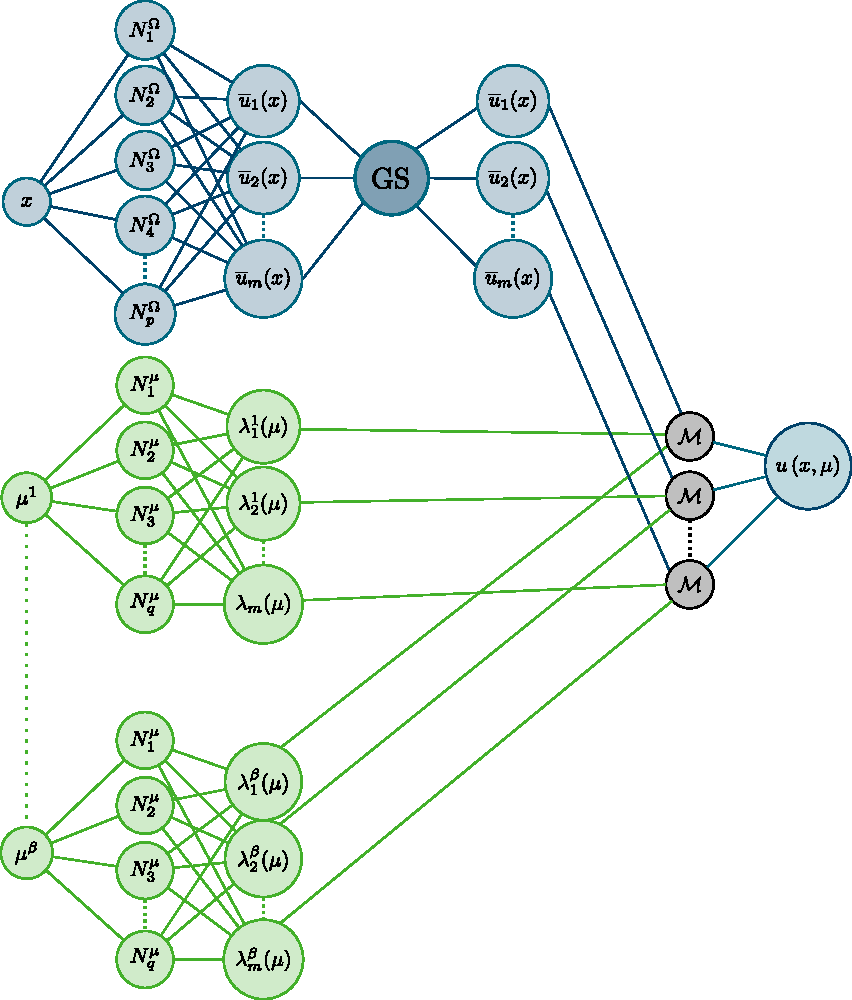
\includegraphics[width = 0.8\textwidth]{Schema/GramSchmidt_NN.pdf}
    \caption{Gram-Schmidt within the HiDeNN-PGD}
    \label{fig:GS_NN}
\end{figure}

\paragraph{This was a bad idea}
It does make sens to orthonomalise the $\left\{ \vect{u}\left( x_i \right) \right\}_{ i \in \llbracket 1, s \rrbracket}$ (with $s$ the number of sampling points) within the NN because it will then depend on the size of the input batches.
Adding a GS algorithm on the \emph{interpolated} space modes (whose size depends on the number of sampling point) only makes sens as a post-process when computing the loss if the training sample is always the same. But this does not seem feasible with more than 1 extra coordinate.

\Rq{The key difference with classical ROM is that not only there are ``Nodally defined'' space modes that lives on the mesh as classically encountered in ROM but there are also the interpolated continuous space modes that are evaluated at the sampling points when evaluating the NN. The latter are the one we play with the most and there interpretation and the operation that can be done on those differ from what is standard on the ``nodal modes'' }